\chapter*{Введение} \label{intro}% * не проставляет номер
\addcontentsline{toc}{chapter}{Введение} % вносим в содержание

В этой работе исследуется совместная работа нескольких агентов с использованием алгоритмов и методов глубокого обучения в 2D игровых средах. В данной работе это имеется в виду, когда изучаются и адаптируются современные алгоритмы и методы глубокого обучения с подкреплением к настройкам игры с несколькими агентами.

Глубокое обучение с подкреплением --- это новая область исследований алгоритмов и методов, которая сочетает в себе обучение с подкреплением и глубокое обучение. Предыдущие работы в основном были направлены на адаптацию глубоких нейронных сетей для усиления алгоритмов обучения. Например, глубокая Q-сеть (Deep Q-network, DQN) \cite{Mnih2015} интегрирует глубокие нейронные сети в Q-обучение --- классический табличный алгоритм обучения с подкреплением. Обученные сети могут играть в различные игры Atari 2600 \cite{Bellemare_2013} лучше человека. Это считается первой успешной попыткой обучить машину играть в видеоигры с прямым визуальным вводом большого размера. Алгоритм глубокого детерминированного градиента политики (deep deterministic policy gradient, \hyperref[acr:ddpg]{DDPG}) \cite{lillicrap2015continuous} --- это ещё один пример использования глубоких нейронных сетей в контексте обучения с подкреплением и непрерывного пространства действий.

Большинство исследований посвящено обучению одного агента. Однако проблемы, связанные с мультиагентным сотрудничеством или конкуренцией, также очень распространены в социальной, экономической и инженерной областях. Игры представляют собой упрощённые версии реальных задач, которые можно сделать идеальными тестовыми площадками для экспериментов. Поэтому в этой работе игровые сценарии используются для изучения алгоритмов глубокого обучения с подкреплением для совместной работы нескольких агентов.

В то же время, в мире очень много задач, которые лучше всего решаются командой, несколькими агентами (см. \hyperref[ch2:ma-algs]{Мультиагентные алгоритмы}).

Было решено изучить мультиагентную составляющую обучения с подкреплением. А именно --- общение. Без общения агентов между собой невозможно достичь хороших результатов. Как в любой командной игре, действия агентов также должны быть скоординированы.

При увеличении количества агентов, а также сложности среды, возрастает сложность обучения агентов, поэтому в данной работе также были изучены различные варианты оптимизации этого процесса.

Исходя из вышеизложенного, была поставлена следующая \textit{цель} - разработка и исследование алгоритмов управления \hyperref[acr:rl]{мультиагентными системами} (МАС) с применением технологий \hyperref[acr:drl]{глубокого обучения с подкреплением}. Для достижения этой цели были поставлены следующие \textit{задачи}:

\begin{enumerate}
	\item Обзор технологии глубокого обучения с подкреплением и её применения в задачах управления;
	\item Обзор методов, алгоритмов управления МАС, их реализаций, практического применения;
	\item Разработка сценариев работы МАС, алгоритмов управления для них;
	\item Реализация сценариев и алгоритмов в игровой среде, экспериментальное исследование алгоритмов, обучения и поведения агентов под влиянием алгоритмов;
	\item Выводы об эффективности алгоритмов в исследованных сценариях, их применимости в прикладных задачах. 
\end{enumerate}

Объект исследования --- это технология обучения с подкреплением.

Предмет исследования --- это применимость обучения с подкреплением к мультиагентным системам.

В данной работе использовались следующие технологии и инструменты:

\begin{itemize}
	\item IDE --- PyCharm Community;
	\item язык программирования - Python;
	\item фреймворк - Tensorflow;
	\item среда для отработки мультиагентных алгоритмов multiagent-particle-envs \cite{multiagent-particle-envs} от компании OpenAI;
	\item базовая реализация алгоритма MADDPG \cite{lowe2017multiagent} от компании OpenAI.
\end{itemize}

В этой работе сперва описываются вопросы исследования, а также сценарии, с которыми выполняются эксперименты.

Затем рассмотриваются теория технологии обучения с подкреплением в целом и мультиагентных систем в частности. Описываются применяемые методы.

Далее описываются эксперименты, их результаты, и делаются выводы.

\chapter{Вводная глава}

\section{Вопросы исследования} \label{intro-questions}

В этой работе исследуются следующие вопросы:
\begin{enumerate}[1.]
	\item Как несколько агентов могут научиться сотрудничать друг с другом во время обучения в определённых игровых сценариях?
	\item Может ли после обучения появиться язык между агентами в определённых игровых сценариях?
	\item Как можно оптимизировать и ускорить процесс обучения?
\end{enumerate}

Сначала будут изучены современные алгоритмы и методы глубокого обучения с подкреплением. Затем будут проведены эксперименты игровых сценариев в модифицированной среде от компании OpenAI \cite{OpenAI-Gym}. Наконец, будут рассмотрены и применены различные приёмы для оптимизации процесса обучения.

\section{Сценарии} \label{intro:sec2}

Чтобы исследовать вышеизложенные вопросы, были использованы некоторые из множества доступных сценариев, где агенты общаются друг с другом и физически перемещаются к определённым целям. Более подробно об этом написано в разделе \hyperref[network-architecture]{Сетевая архитектура}.

Некоторые из сценариев являются точными копиями экспериментов, проведённых в недавней работе \cite{lowe2017multiagent}, а другие представляют собой новые сценарии, которые расширяют исходные с целью дальнейшего изучения многоагентного сотрудничества и коммуникации.

\subsection{Сценарий 1. Simple Speaker Listener} \label{intro:ssl}

В этом сценарии есть три ориентира, представленные как красные, зелёные и синие ориентиры, как показано на \firef{fig-intro-ssl}. Два агента с разными функциями должны сотрудничать для достижения общей цели. \textit{Говорун} (серый агент) не может двигаться, но видит цвет цели и может говорить с другим агентом. \textit{Слушатель} (отображаемый таким же цветом, что и его цель) видит все ориентиры и их цвета (но не видит собственный цвет, т.е. не знает, какой из объектов является его целью), а также слышит \textit{говоруна} и пытается перейти к правильному ориентиру. Более подробные настройки среды этого сценария можно найти в разделе \hyperref[exp-ssl]{Эксперименты: Сценарий 1. Simple Speaker Listener}.
% TODO хардкод номера главы

\begin{figure}[ht!] 
	\center
	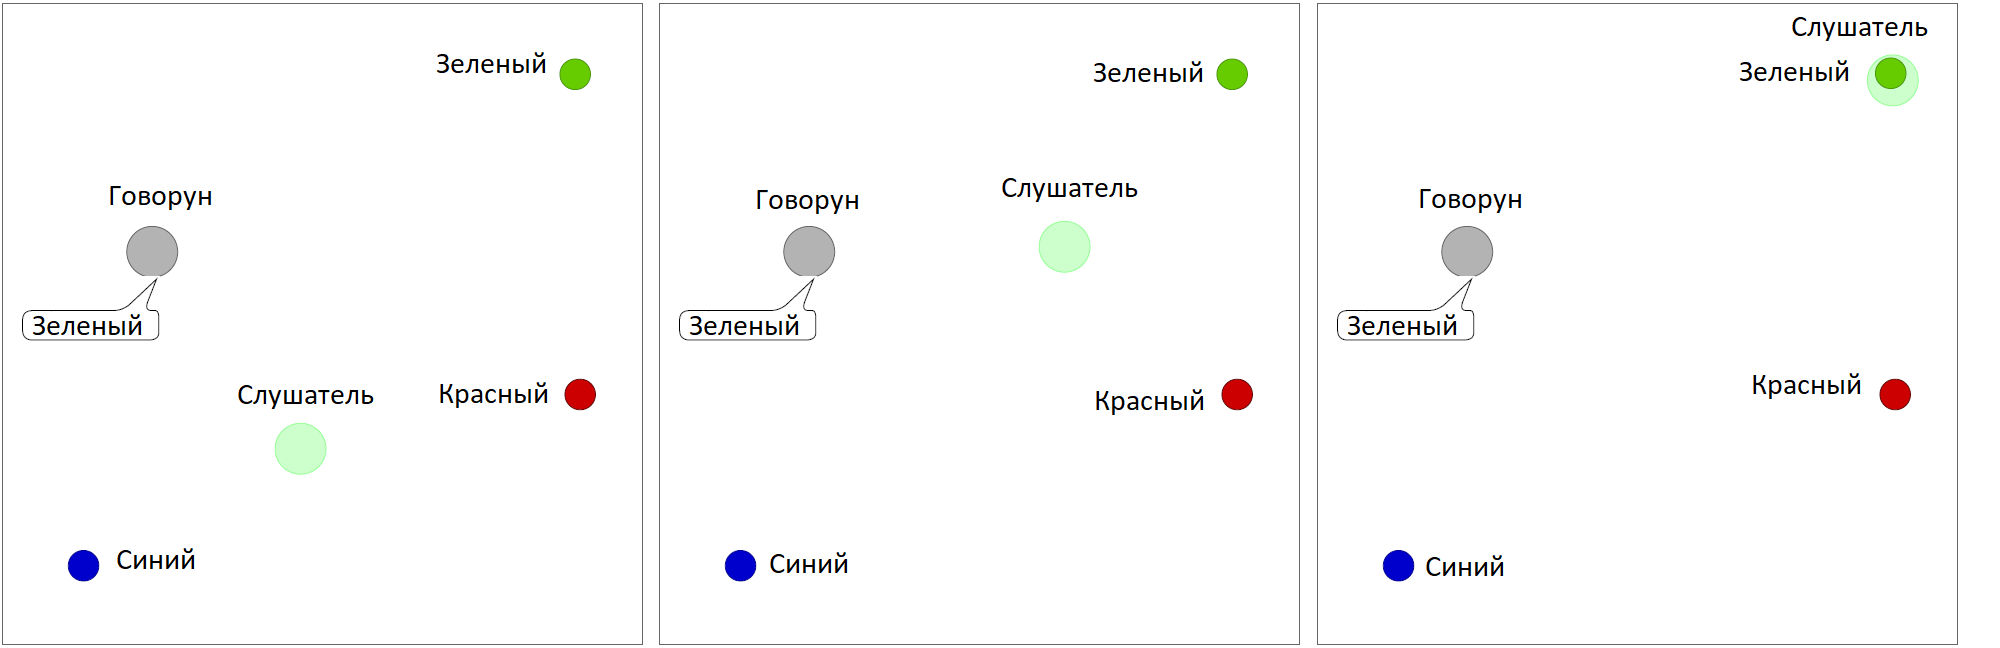
\includegraphics [scale=0.41] {my_folder/images/intro/ssl.png}
	\caption{Сценарий 1. \textit{Simple Speaker Listener}. Скриншоты слева направо показывают этапы игрового эпизода. \textit{Говорун} (серый) выдаёт коммуникационное действие, представляющее «зелёный», а \textit{слушатель} слушает сообщение \textit{говоруна} и направляется к цели}
	\label{fig-intro-ssl}
\end{figure}

\begin{figure}[ht!] 
	\center
	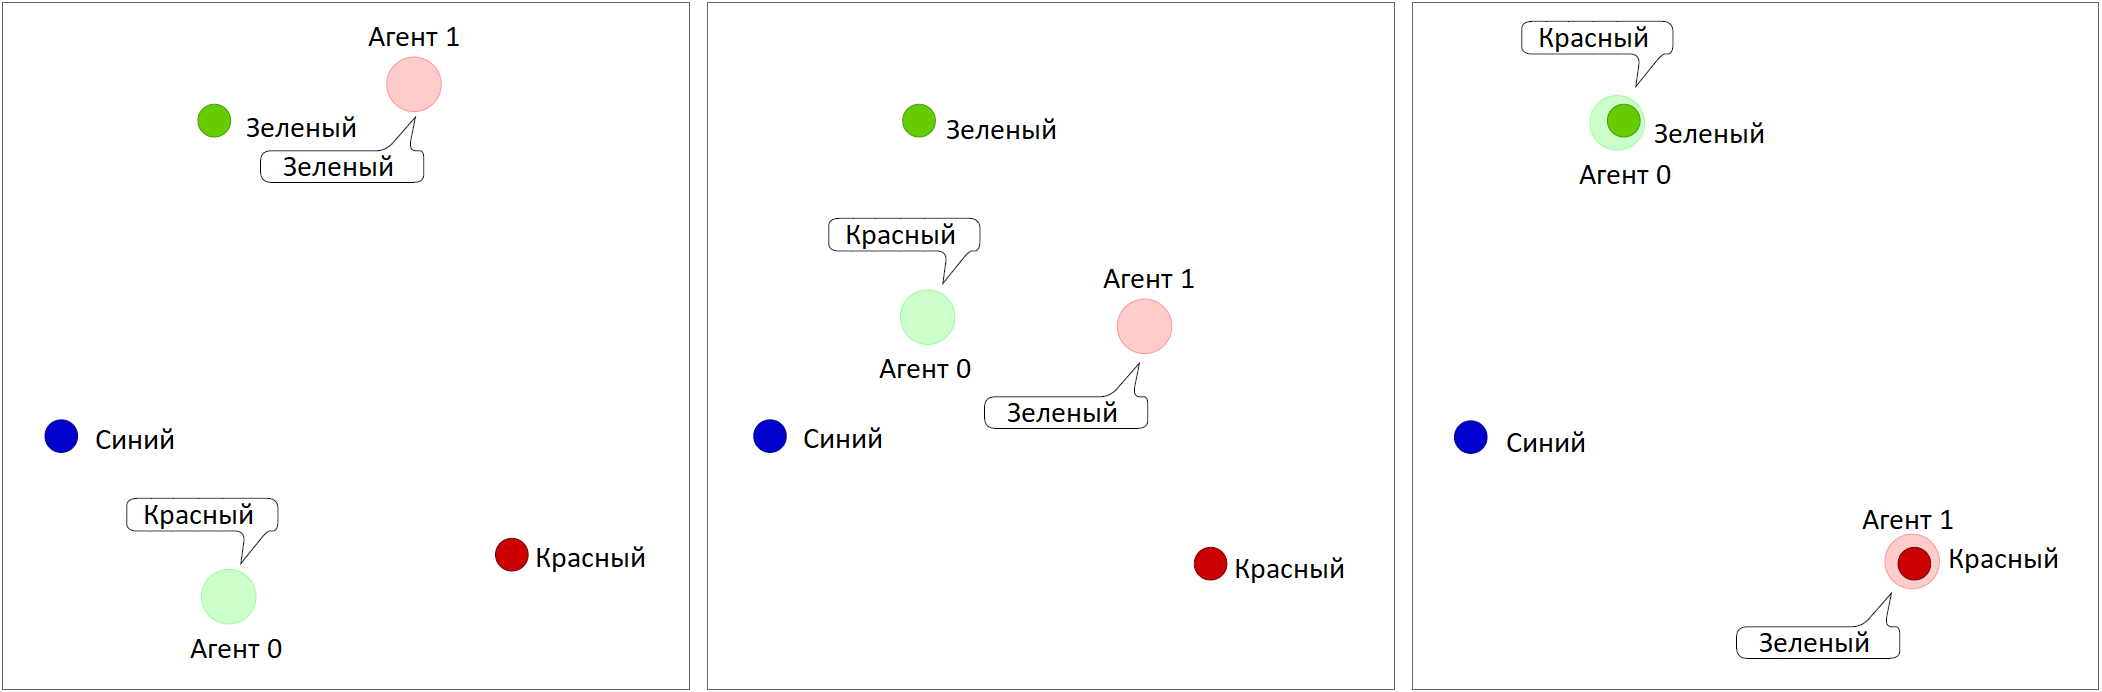
\includegraphics [scale=0.38] {my_folder/images/intro/sr.png}
	\caption{Сценарий 2: \textit{Simple Reference}. В этом эпизоде агент 0 (отображаемый в том же цвете, что и его целевой ориентир) выдаёт коммуникационное действие, представляющее «красный», и слушает агента 1. А агент 1 (отображается в том же цвете, что и его целевой ориентир) слушает и издаёт «зелёный» для Агента 0. Скриншоты слева направо показывают, как ведут себя два агента в соответствии с оптимальными политиками, слушая друг друга и перемещаясь к целям}
	\label{fig-intro-sr}
\end{figure}

\subsection{Сценарий 2. Simple Reference} \label{intro-sr}

Этот сценарий расширяет предыдущий, поскольку оба агента являются одновременно и \textit{говорунами} и \textit{слушателями}. Ориентиры остаются прежними, отображаются как три разноцветных объекта, (как изображено на \firef{fig-intro-sr}). Каждый из двух агентов пытается достичь своего целевого ориентира, который известен только другому агенту. Таким образом, он должен научиться сообщать другому агенту его цель и перемещаться к своей собственной. Что отличает сценарий от двух копий сценария \textit{Simple Speaker Listener}, так это то, что единое общее вознаграждение, присуждаемое агентам, основано на общей производительности. Таким образом, агенты должны выяснить, что идёт хорошо, а что нет. Настройка среды подробно описана в разделе \hyperref[exp-sr]{Эксперименты: Сценарий 2. Simple Reference}.
 % TODO: сверить имя главы

\subsection{Сценарий 3. Simple World Communication} \label{intro-swc}

В этом сценарии есть \textit{хорошие агенты} (зелёные) и их противники – \textit{преследователи} (красные). Также есть \textit{препятствия} (чёрные), \textit{леса} (зелёные) и \textit{еда} (зелёные). Один из преследователей – \textit{лидер} (тёмно-красный).

\textit{Хорошие агенты} награждаются за то, что приближаются к \textit{еде} и наказываются, когда касаются преследователей.

\textit{Преследователи} награждаются за касание хороших агентов.

\textit{Лес} скрывает агентов от преследователей. \textit{Лидер} видит агентов даже в лесу (cм. \firef{fig:swc}).

\begin{figure}[ht!] 
	\center
	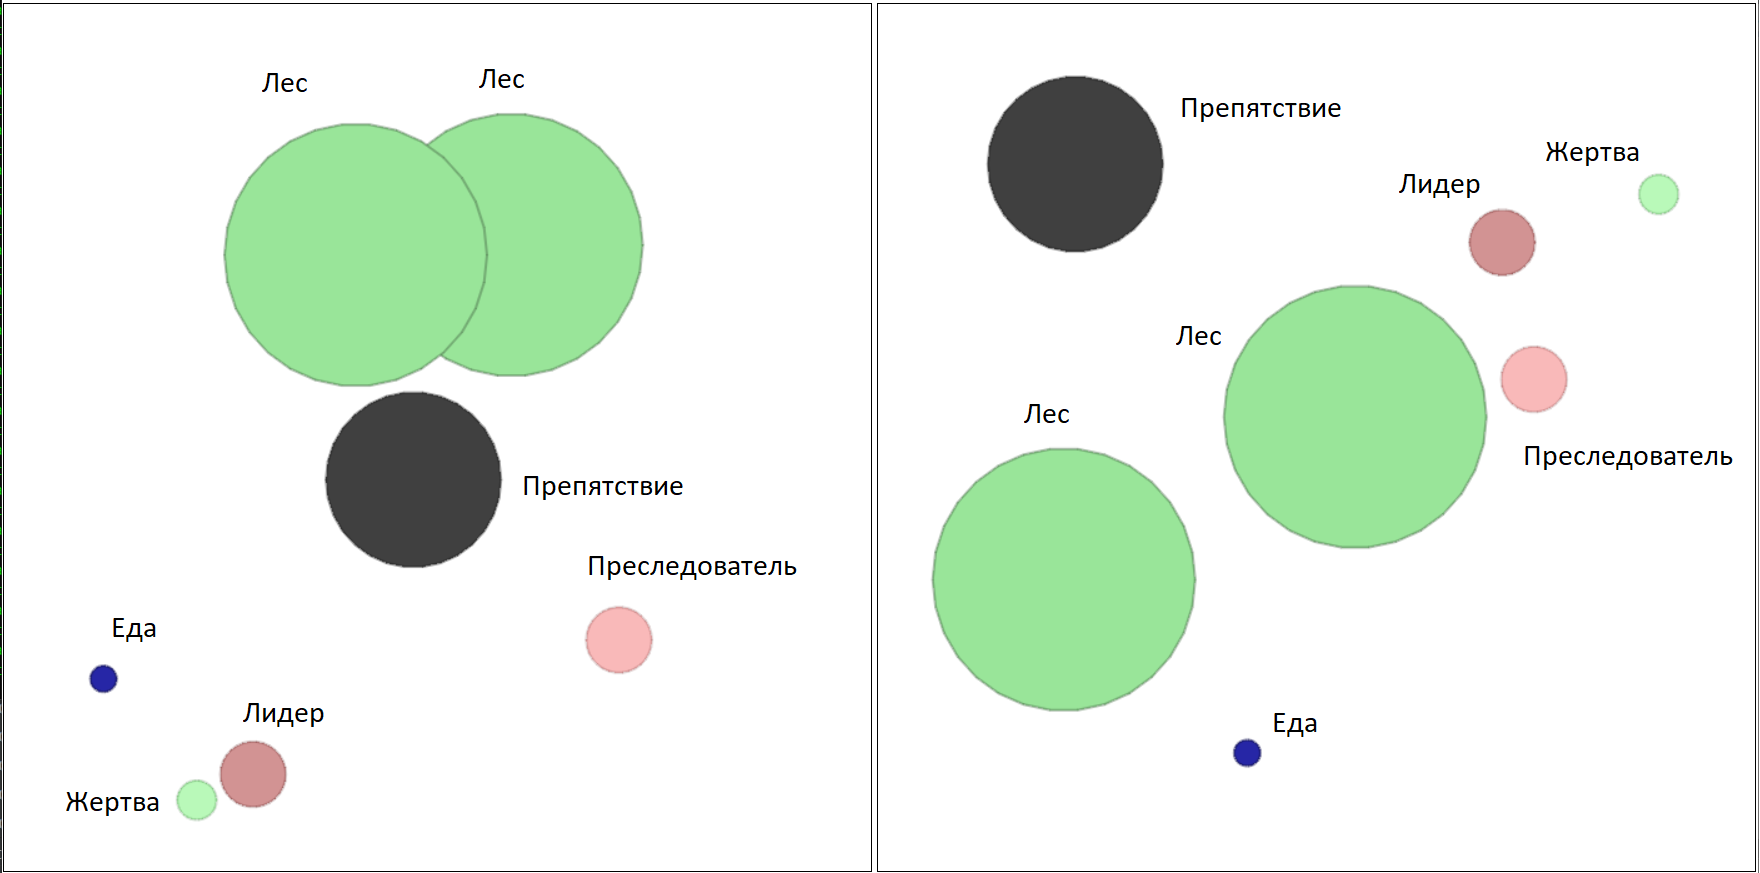
\includegraphics [scale=0.41] {my_folder/images/intro/swc.png}
	\caption{Сценарий Simple World Communication, жертва избегает преследователей, и, по возможности, приближается к еде, преследователи догоняют жертву}
	\label{fig:swc}  
\end{figure}

Более подробное описание и настройки можно найти в разделе \hyperref[exp-swc]{Эксперименты: Сценарий 3. Simple World Communication}.

\subsection{Сценарий 4: Simple Tag} \label{intro-st}

В этом сценарии есть \textit{хорошие агенты} (зелёные) и их противники – \textit{преследователи} (красные). Так же есть \textit{препятствие} (чёрное).

\textit{Хорошие агенты} наказываются, когда касаются \textit{преследователей}.

\textit{Преследователи} награждаются за касание \textit{хороших агентов}.

\textit{Преследователей} больше, но у \textit{жертвы} больше скорость. Теоретически, \textit{преследователи} должны выработать политику, при которой они окружают жертву или другие подобные приёмы. \textit{Жертва} должна не позволять загнать себя в угол.

Также данный сценарий был немного модифицирован --- была добавлена граница по периметру поля, которая не даёт агентам покинуть видимую часть.

\begin{figure}[ht!] 
	\center
	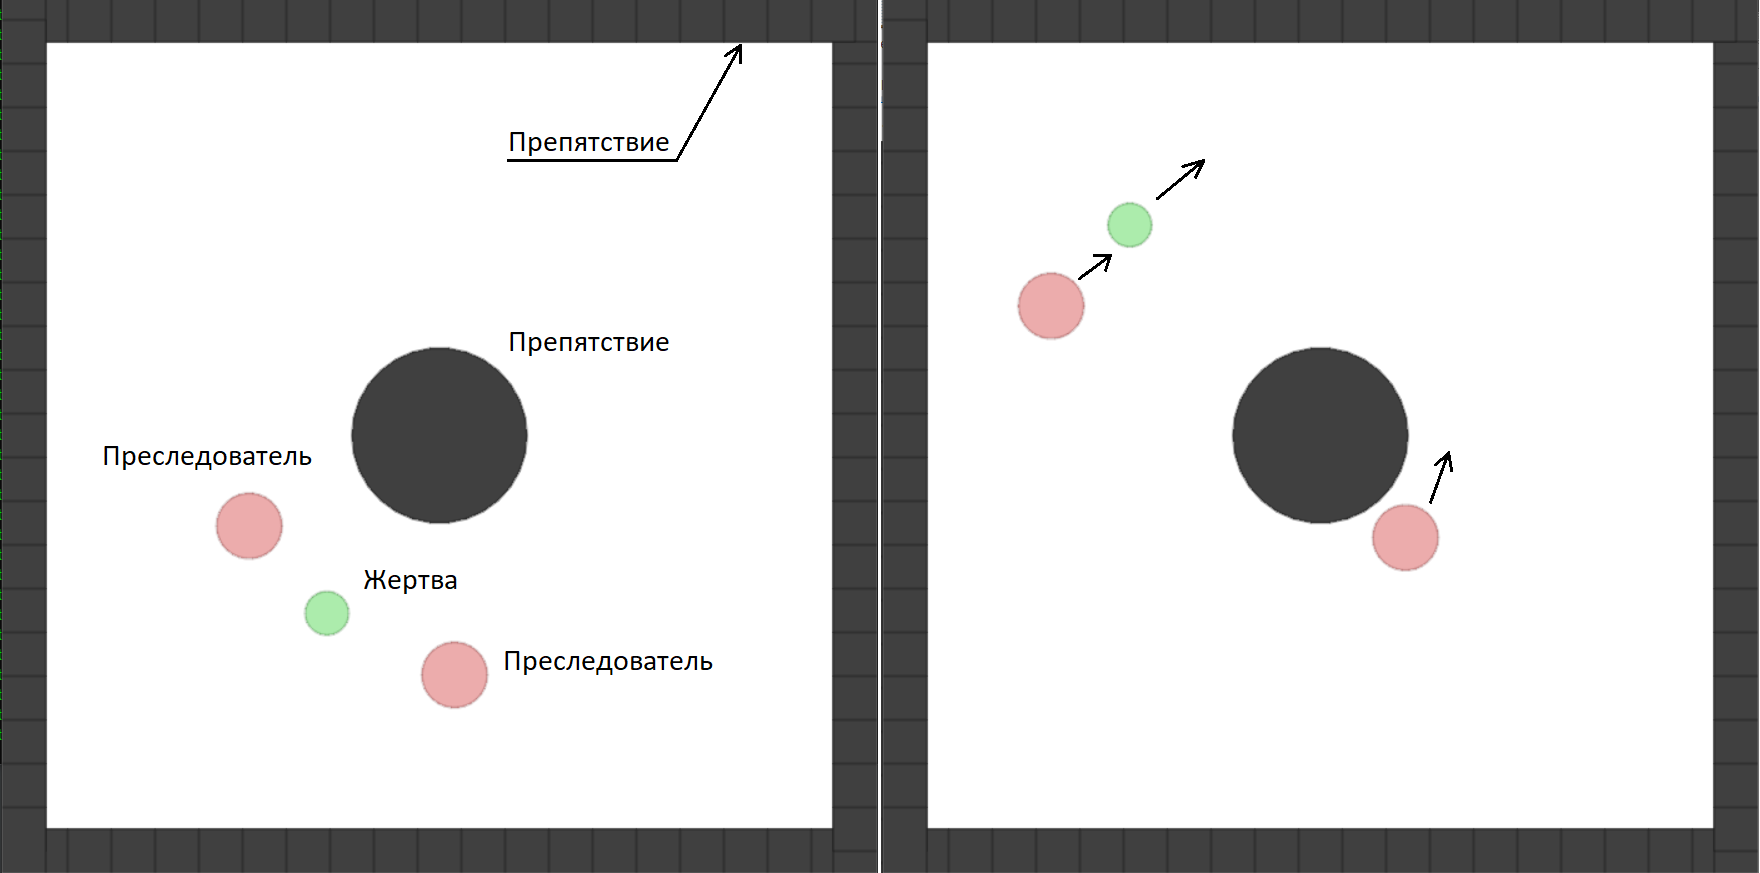
\includegraphics [scale=0.41] {my_folder/images/intro/st.png}
	\caption{Сценарий Simple Tag. \textit{Жертва} избегает \textit{преследователей}. На правом скриншоте правый преследователь превентивно обходит \textit{препятствие} справа и движется в ту же область, что и \textit{жертва}}
	\label{fig:st}  
\end{figure}

Более подробное описание и настройки можно найти в разделе \hyperref[exp-st]{Эксперименты: Сценарий 4. Simple Tag}.

\section{Практическая значимость} \label{intro:sec3}

Проект сосредоточен на обучении нескольких агентов совместной работе с использованием глубокого обучения в игровой среде. Результаты исследования могут быть дополнительно разработаны и широко использованы во многих практических реальных приложениях в области экономики, управления, техники и т.д. Например, он может применяться в робототехнике, к автономным транспортным средствам, производственным линиям, фондовым рынкам и т.д.

Перед применением в этих областях алгоритмы и методы, которые исследуются и разрабатываются в этой работе, должны быть хорошо протестированы и проверены, поскольку эти приложения непосредственно влияют на безопасность человека, социальную и финансовую безопасность. В долгосрочной перспективе применение мультиагентных алгоритмов приведёт к появлению всё большего числа автономных систем во многих областях.


%% Вспомогательные команды - Additional commands
%\newpage % принудительное начало с новой страницы, использовать только в конце раздела
%\clearpage % осуществляется пакетом <<placeins>> в пределах секций
%\newpage\leavevmode\thispagestyle{empty}\newpage % 100 % начало новой строки
